\documentclass[c,11pt,xcolor=dvipsnames, aspectratio=169]{beamer}

%Insert number of slides
\beamertemplatenavigationsymbolsempty
\addtobeamertemplate{navigation symbols}{}{%
    \usebeamerfont{footline}%
    \usebeamercolor[fg]{footline}%
    \hspace{1em}%
    \insertframenumber/\inserttotalframenumber
}

% Redefine itemize
\def\labelitemi{--}


%Define colors useful for presentation
\definecolor{UniBlue}{RGB}{0,102,204}
\definecolor{UniOrange}{RGB}{255,128,0}
\definecolor{mygreen}{RGB}{120,190,33}
\newcommand{\green}[1]{\textcolor{ForestGreen}{#1}}

%\definecolor{color1}{HTML}{B3E2CD}
%\definecolor{color2}{HTML}{FDCDAC}
%\definecolor{color3}{HTML}{CBD5E8}
%\definecolor{color4}{HTML}{F4CAE4}
%\definecolor{color5}{HTML}{E6F5C9}

%\definecolor{color1}{HTML}{66C2A5}
%\definecolor{color2}{HTML}{FC8D62}
%\definecolor{color3}{HTML}{8DA0CB}
%\definecolor{color4}{HTML}{E78AC3}
%\definecolor{color5}{HTML}{A6D854}

\definecolor{color1}{HTML}{1B9E77}
\definecolor{color2}{HTML}{D95F02}
\definecolor{color3}{HTML}{7570B3}
\definecolor{color4}{HTML}{E7298A}
\definecolor{color5}{HTML}{66A61E}


\setbeamercolor{title}{fg=color1}
\setbeamercolor{frametitle}{fg=color1}
\setbeamercolor{structure}{fg=color3}
\setbeamercolor{footline}{fg=black}
\setbeamercolor{caption name}{fg=black}
\setbeamercolor{bibliography item}{fg=black}
\setbeamercolor*{bibliography entry title}{fg=black}
\setbeamercolor*{bibliography entry author}{fg=black}
\setbeamercolor*{bibliography entry location}{fg=black}
\setbeamercolor*{bibliography entry note}{fg=black}


\setbeamertemplate{section in toc}[sections numbered]
\setbeamertemplate{caption}[numbered]
\setbeamertemplate{bibliography item}{\insertbiblabel}

%Additional packages
\usepackage{blkarray}
\usepackage{amsmath}
\usepackage{amsfonts}
\usepackage{amssymb}
\usepackage{algorithm2e}
\usepackage{appendixnumberbeamer}
\usepackage{pgfplots}
\usepgfplotslibrary{groupplots,dateplot}
\usetikzlibrary{patterns,shapes.arrows}
\pgfplotsset{compat=newest}
\usepackage{multimedia}
\usepackage{media9}
\usepackage{pbox}
\usepackage{multirow}
\usepackage[makeroom]{cancel}
\usepackage[export]{adjustbox}
\usepackage{tabularx}
\usepackage{caption}
\usepackage{xcolor}
\usepackage{pgfplotstable,filecontents}
\usepackage{listings}
\usepackage{enumitem}
\usepackage{algorithmic}
\usepackage{bm}
\usepackage{tikz}
\usetikzlibrary{shapes.geometric, arrows}

\tikzstyle{process} = [rectangle, rounded corners, minimum width=3cm, minimum height=1cm, text centered, draw=black, fill=color1]
\tikzstyle{arrow} = [thick,->,>=stealth]

%Shading text: useful to highlight information
\usepackage{framed, color}
\definecolor{shadecolor}{RGB}{220,220,220}
\usepackage{makecell}

\usepackage{subcaption}
%Define logos for subojectives
% \newcommand{\logoso1}{\setbeamertemplate{logo}{\includegraphics[width=0.1\textwidth]{images/so1.png}}
\def\mathunderline#1#2{\color{#1}\underline{{\color{black}#2}}\color{black}}


\usepackage{siunitx}

% Add an outline slide at the beginning of each new section
\AtBeginSection[]
{
	{
		\setbeamertemplate{footline}{} %this line removes slides numbers
		\begin{frame}[noframenumbering]
			\frametitle{Outline}
			\tableofcontents[currentsection]
		\end{frame}
	}
}




%-------------------------
% Title page
%-------------------------
% Details for title page
% Commenting the line below will make the title page centered
\setbeamertemplate{title page}[default][left,colsep=-4bp,rounded=true,shadow=\beamer@themerounded@shadow]

\title{\textbf{Volume-Averaged Navier-Stokes Equations}}
\subtitle{A not so short introduction to the theory and application}
\author{Bruno \textit{problembär} Blais}


% Logo of the laboratory and the university
\titlegraphic{
\includegraphics[width=4.2cm]{../../logos/chaos_logo_black_without_bkg.png}\hspace*{6.8cm}~%
   
\includegraphics[width=3cm]{../../logos/Polytechnique_signature-RGB-droite_ENG.png}
}



\begin{document}

% Title slide
{
\setbeamertemplate{footline}{} %this line removes slide number
\begin{frame}[noframenumbering]
  \titlepage
\end{frame}
}

%%Contents slide
\begin{frame}
	\frametitle{\textbf{Outline}}
	\tableofcontents
\end{frame}

\section{What do the VANS equation model?}


\begin{frame}{\textbf{Volume-Averaged Navier-Stokes (VANS) equations}}
	\visible<1->
	{\begin{shaded}
			The \textbf{Volume-Averaged Navier-Stokes} are used to simulate flows with spatially ($\bm{x}$) and temporally ($t$) varying void fraction ($\epsilon$)
	\end{shaded}}
	
	\begin{minipage}[t]{0.48\linewidth}
		%\visible<2->
		{
			\begin{block}{Used in the following models:}
				\begin{itemize}
					\item Two-fluid models
					\item Unresolved CFD-DEM
					\item Porous media flow
				\end{itemize}
			\end{block}
		}
	\end{minipage}%
	\hfill%
	%
	\begin{minipage}[t]{0.48\linewidth}
		%\visible<3->
		{
			\begin{block}{For many applications:}
				\begin{itemize}
					\item Fluidized and spouted-bed reactors
					\item Free surface flows in containers
					\item DNS of particle-laden flow
					\item Mixing in stirred tanks 
					\item Flow in porous media
				\end{itemize}
			\end{block}
		}
	\end{minipage}
\end{frame}


\begin{frame}{\textbf{VANS equations}}
\begin{block}{Mass conservation:}
\[
\partial_t \epsilon + \partial_i (\epsilon u_i) = 0
\]
\end{block}

\begin{block}{Momentum conservation:}
	\[
	\partial_t \left(\epsilon u_i\right) + \partial_j (\epsilon u_i u_j) = \frac{\epsilon}{\rho} \partial_i p + \partial_j \left(\epsilon \tau_{ij}\right) + \epsilon g_i
	\]
	\end{block}

	with:
	\begin{itemize}
	\item $\epsilon$ the void fraction
	\item $u_i$ the velocity
	\item $\rho$ the density
	\item $p$ the pressure
	\item $\tau_{ij}$ the deviatoric stress tensor
	\item $g_i$ the body acceleration per unit volume (e.g. gravity)
	\end{itemize} 


\end{frame}

\begin{frame}
	\frametitle{\textbf{What do these equations model? An example}}
	
	%\vspace{0.1cm}
	\begin{columns}[c]
		\begin{column}{0.5\textwidth}
			Fluid flows through a channel with packed particles in the middle.
			\begin{itemize}
				\item The void fraction varies in space 
				\item If the particle fluidize, the void fraction also varies in time
			\end{itemize}
			\end{column}
		\begin{column}{0.5\textwidth}
			\vspace*{-\baselineskip}
			\begin{center}
				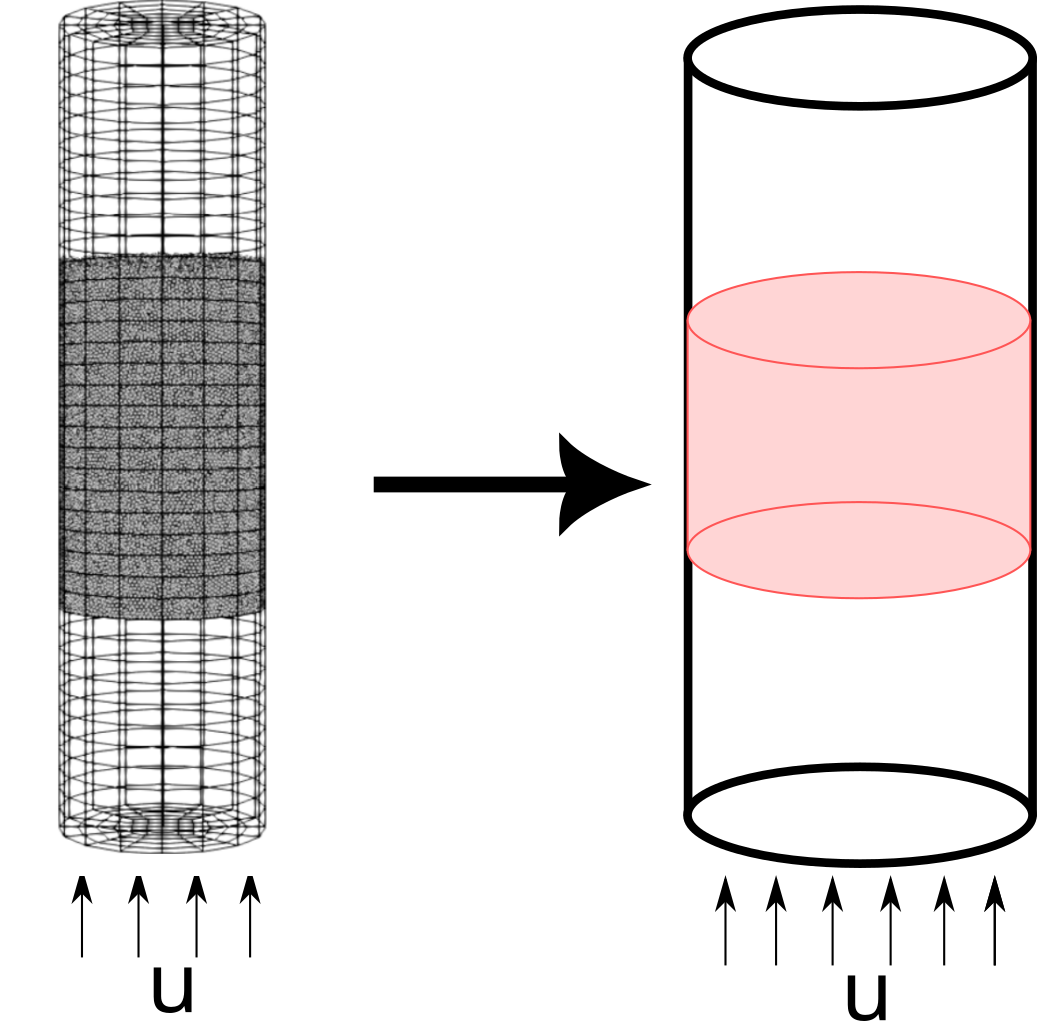
\includegraphics[width=0.9\textwidth]{images/vans_cylinder.png}
			\end{center}
		\end{column}
	\end{columns}
\end{frame}

\begin{frame}
	\frametitle{\textbf{A simplified representation of this problem}}
	
Without loss of generality, let's assume steady state and $\epsilon=\epsilon(z)$ such that:
\[
\epsilon(z) = \begin{cases}
	1 & \text{if } z < z_0 \\
	0.5 & \text{if } z \in[z_0, z_1] \\
	1 & \text{if } z > z_1
\end{cases}
\]
And that the velocity at the inlet is uniform in the $xy$ plane and constant ($u$). Then, from mass conservation, we have:
\[
\partial_t \epsilon + \partial_z (\epsilon u_z) = 0
\]
Since we are in steady state, we have $\partial_t \epsilon = 0$, and thus:
\[
\partial_z (\epsilon u_z) = 0
\]
This means that $u_z$ is:
\[
	\epsilon(z) = \begin{cases}
		u & \text{if } z < z_0 \\
		2u & \text{if } z \in[z_0, z_1] \\
		u & \text{if } z > z_1
	\end{cases}
\]

\end{frame}

\begin{frame}
	\frametitle{\textbf{Graphical representation of the solution}}

		%\vspace{0.1cm}
		\begin{columns}[c]
			\begin{column}{0.5\textwidth}
				Variation imply of $\epsilon$ create:
				\begin{itemize}
					\item Acceleration and/or deceleration of the fluid
					\item \textbf{Should it generate stresses?}
					\item \textbf{Where is this momentum coming from?}
				\end{itemize}
				\end{column}
			\begin{column}{0.5\textwidth}
				\vspace*{-\baselineskip}
				\begin{center}
					%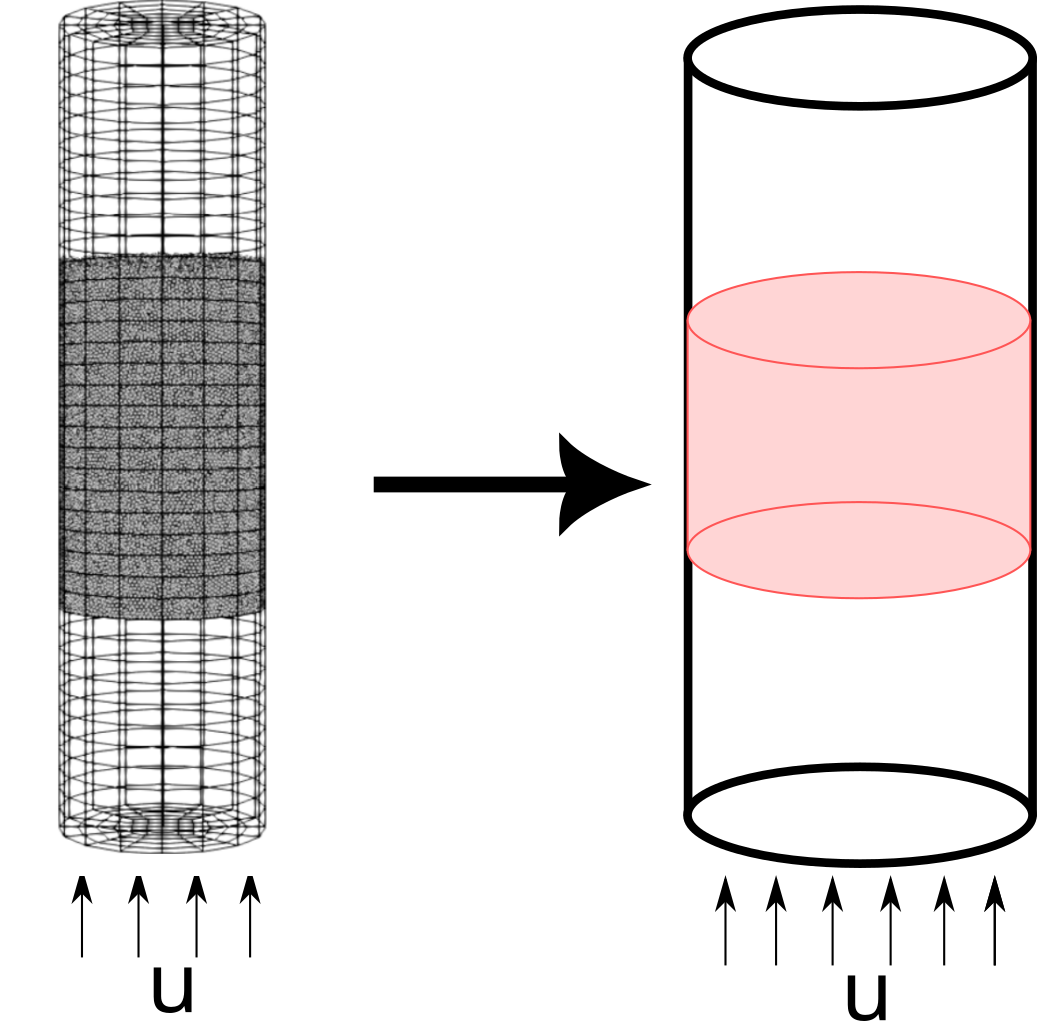
\includegraphics[width=0.9\textwidth]{images/vans_cylinder.png}
				\end{center}
			\end{column}
		\end{columns}
\end{frame}


\section{Origin of the equations}


\section{A straightforward implementation}

\section{An alternative perspective}

\section{Conclusion: the end}

\begin{frame}{Conclusions}
\begin{block}{GIT and version control}
	\begin{itemize}
	\item Essential if you want to work as part of a team
	\item Allows you to track every change and go back in time (e.g. git bissect)
	\item Allows you to share your code with who you want in a safe and controllable way.
	\end{itemize}
\end{block}

\begin{block}{You need to change the way you work}
	\begin{itemize}
	\item When you start a new feature, create a branch and work on it.
	\item Aim for small features, once they are complete, merge them.
	\item Don't be afraid of criticism, getting comments is a good way to get better.
	\end{itemize}
\end{block}
\end{frame}


\begin{frame}{Advices for the future}

	\begin{block}{Above all things, using git requires discipline}
		\begin{itemize}
		\item If you can name an idea or a change, it should be a branch and a pull request.
		\item Ensure you have ways to test your changes. Automating these tests is easier than you think (e.g. use continuous integration)
		\item Write clear commit messages and pull request messages. It is a small time investment that can save you a lot of time and it structures your ideas.
		\item Do not be afraid of failing or making mistake, git enables you to go back in time, so you CAN do large-scale refactoring.
		\end{itemize}
	\end{block}

	\begin{block}{There is more to git...}
		\begin{itemize}
		\item Rebase
		\item Cherry-picking
		\item Squashing
		\item ... (many other things I do not know)
		\end{itemize}
	\end{block}

\end{frame}

\end{document}